\section{Results}

\subsection{Execution Time}
\begin{figure}[H]
    \centering
    \includegraphics[width=.6\textwidth]{plots/run-2/time/all_benchmarks.pdf}
    \caption{Overview execution time}
    \label{fig-exec-time-overview}
\end{figure}

\begin{figure}[H]
    \centering
    \includegraphics[width=.6\textwidth]{plots/run-2/time/benchmark_cata_sum.pdf}
    \caption{Execution time for Cata Sum}
    \label{fig-exec-time-cata-sum}
\end{figure}

\begin{figure}[H]
    \centering
    \includegraphics[width=.6\textwidth]{plots/run-2/time/benchmark_generic_cata_sum.pdf}
    \caption{Execution time for Generic Cata Sum}
    \label{fig-exec-time-gen-cata-sum}
\end{figure}

\begin{figure}[H]
    \centering
    \includegraphics[width=.6\textwidth]{plots/run-2/time/benchmark_incremental_cata_sum.pdf}
    \caption{Execution time for Incremental Cata Sum}
    \label{fig-exec-time-inc-cata-sum}
\end{figure}


\subsection{Memory Usage}
\begin{figure}[H]
    \centering
    \includegraphics[width=.6\textwidth]{plots/run-2/memory/all_benchmarks.pdf}
    \caption{Overview memory usage}
    \label{fig-bytes-all-overview}
\end{figure}

\begin{figure}[H]
    \centering
    \includegraphics[width=.6\textwidth]{plots/run-2/memory/benchmark_cata_sum.pdf}
    \caption{Memory usage for Cata Sum}
    \label{fig-bytes-all-cata-sum}
\end{figure}

\begin{figure}[H]
    \centering
    \includegraphics[width=.6\textwidth]{plots/run-2/memory/benchmark_generic_cata_sum.pdf}
    \caption{Memory usage for Generic Cata Sum}
    \label{fig-bytes-all-gen-cata-sum}
\end{figure}

\begin{figure}[H]
    \centering
    \includegraphics[width=.6\textwidth]{plots/run-2/memory/benchmark_incremental_cata_sum.pdf}
    \caption{Memory usage for Incremental Cata Sum}
    \label{fig-bytes-all-inc-cata-sum}
\end{figure}

\subsection{Comparison Memory Strategies}
\begin{figure}[H]
    \centering
    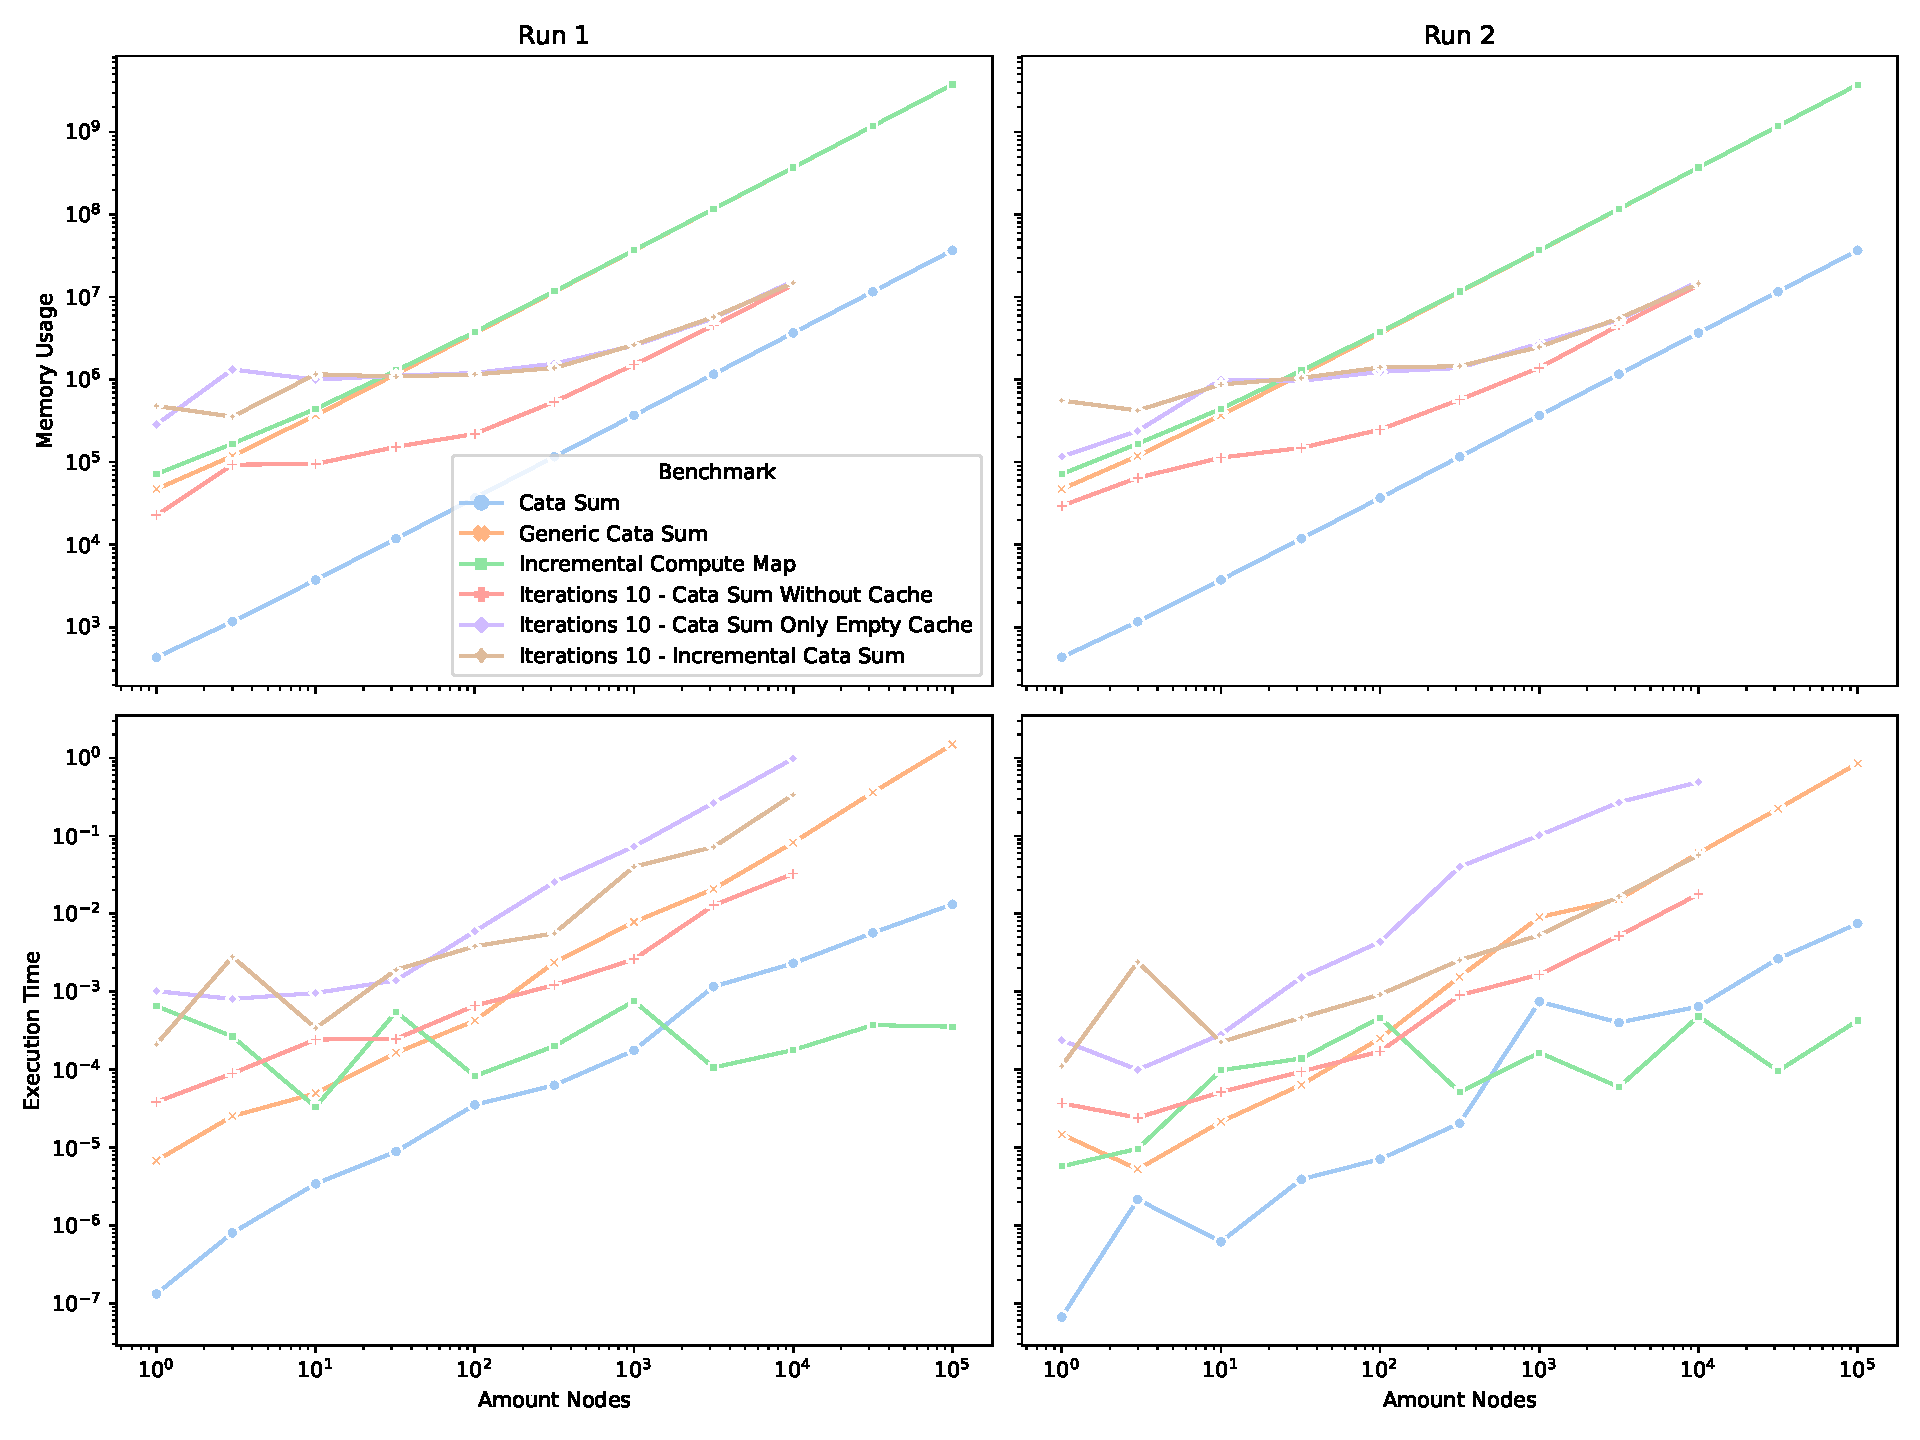
\includegraphics[width=.9\textwidth]{plots/run-2_run-1/comparison_benchmarks.pdf}
    \caption{Comparison Memory Strategy}
    \label{fig-comp-mem-strat}
\end{figure}